% vim: tw=82
\chapter{The Castle}

The default program launcher is the Castle. You can use this launcher to access
all of your installed programs, as well as manage your favorite ones in an
easy-to-access place. This will be the center of operations for your calculator.
You will use the program launcher to get to the math program, the graphing
program, and everything else.

\begin{figure}[ht!]
    \centering
    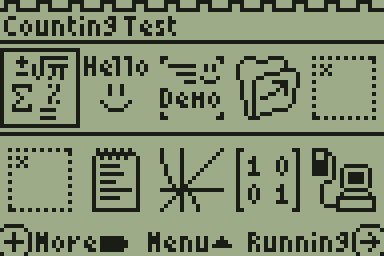
\includegraphics[width=0.8\textwidth,natwidth=384,natheight=256]{castle-front}
\end{figure}

\section{Common Programs}

You are able to ``pin'' up to 10 programs to your Castle's home screen. A
reasonable set of defaults is pinned for you when you first install KnightOS. To
open a program, press \textbf{ENTER} or \textbf{2ND}. You may unpin the program by
pressing \textbf{DEL}, or by replacing it with another program.

\section{Power Management}

To turn off your calculator, you may press \textbf{F3} to open the power menu.
The following choices are available:

\begin{description}
    \item[Sleep] Power off the calculator without closing any programs.
    \item[Shut Down] Close all programs and power off.
    \item[Restart] Close all programs and reboot.
\end{description}

\section{All Programs}

To access a list of all programs installed on your calculator, press \textbf{F1}.
You may press \textbf{F5} with any of these programs highlighted to pin that
program to your home screen.

\section{Customizing the Castle}

You can customize the castle in a number of ways. The most drastic change could be
to install another launcher entirely. Since KnightOS is flexible and all of the
pieces are decoupled from each other, you can easily install an alternative
launcher. Of course, a less ambitious user might simply want to reorganize the
home screen or change the icons.
